\chapter{Specification and Design Decisions}

This chapter explains how \projectname{} moved from the WR1 requirements baseline into a narrower Unity prototype. The focus is traceability rather than redesign: what WR2 inherits, what it simplifies, and what it defers so the prototype remains demonstrable.

\section{Requirements Validation}

Table~\ref{tab:wr1-wr2-traceability} makes the WR1 to WR2 relationship explicit. It distinguishes direct inheritance, implementation-driven narrowing, and visible deferred work.

\providecommand{\tracecell}[2]{\parbox[t]{#1}{\RaggedRight #2}}

\begingroup
\scriptsize
\setlength{\tabcolsep}{4pt}
\begin{longtable}{@{}lllll@{}}
\caption{WR1 to WR2 requirements traceability}
\label{tab:wr1-wr2-traceability}\\
\toprule
\textbf{WR1 baseline} & \textbf{WR2 status} & \textbf{Reason for change} & \textbf{Evidence source} & \textbf{RE conformance} \\
\midrule
\endfirsthead
\toprule
\textbf{WR1 baseline} & \textbf{WR2 status} & \textbf{Reason for change} & \textbf{Evidence source} & \textbf{RE conformance} \\
\midrule
\endhead
\bottomrule
\endfoot
\bottomrule
\endlastfoot
\tracecell{0.17\textwidth}{WR1 personas and first-battle scenarios for casual strategy players.} &
\tracecell{0.14\textwidth}{\textbf{Inherited}} &
\tracecell{0.16\textwidth}{WR2 still validates the same audience and first-use situations instead of redefining them.} &
\tracecell{0.18\textwidth}{WR1 report; walkthrough note; prototype screenshots.} &
\tracecell{0.15\textwidth}{Yes. Validation still follows the user-facing concerns elicited in WR1.} \\
\tracecell{0.17\textwidth}{Core battle loop: turn start, draw, unit/card/target selection, enemy turn, and battle check.} &
\tracecell{0.14\textwidth}{\textbf{Inherited}} &
\tracecell{0.16\textwidth}{This is the minimum playable slice needed to demonstrate the WR1 concept without widening scope.} &
\tracecell{0.18\textwidth}{Snapshot verification; first-pass script note; runtime scene.} &
\tracecell{0.15\textwidth}{Yes. WR2 implements the same central interaction flow and checks it against runtime evidence.} \\
\tracecell{0.17\textwidth}{6x6 board, battle UI, hand zone, turn controls, and starter cards \texttt{Move}, \texttt{Strike}, \texttt{Guard}, and \texttt{Push}.} &
\tracecell{0.14\textwidth}{\textbf{Inherited}} &
\tracecell{0.16\textwidth}{The starter content stayed narrow so the tactics loop remained readable and testable within coursework time.} &
\tracecell{0.18\textwidth}{Snapshot verification; architecture constraints note; Figures~\ref{fig:prototype-evidence}--\ref{fig:prototype-board}.} &
\tracecell{0.15\textwidth}{Yes. WR2 preserves the functional baseline promised for the demo combat scenario.} \\
\tracecell{0.17\textwidth}{Readable feedback, onboarding cues, and understandable turn results as non-functional usability goals.} &
\tracecell{0.14\textwidth}{\textbf{Modified}} &
\tracecell{0.16\textwidth}{WR2 keeps prompts, highlights, HP visibility, guard state, logs, and text outcomes, but tutorial depth and presentation polish were reduced for stability.} &
\tracecell{0.18\textwidth}{Walkthrough note; EditMode test note; merged PR \#5.} &
\tracecell{0.15\textwidth}{Yes, in partial form. The simplification is explicit rather than hidden.} \\
\tracecell{0.17\textwidth}{WR1 system model and architecture expectations around turn flow, grid logic, units, cards, and UI.} &
\tracecell{0.14\textwidth}{\textbf{Modified}} &
\tracecell{0.16\textwidth}{The responsibility split stayed, but implementation was narrowed to one battle scene, one shared \texttt{UnitController}, one explicit \texttt{CardResolver}, deterministic \texttt{EnemyAI}, and a prototype-first UI path.} &
\tracecell{0.18\textwidth}{Architecture constraints note; first-pass scripts; implementation decisions; Figures~\ref{fig:architecture} and \ref{fig:module-map}.} &
\tracecell{0.15\textwidth}{Yes. The architecture remains traceable to WR1 and the scope-control decisions are named explicitly.} \\
\tracecell{0.17\textwidth}{Organisational requirement for repository-based teamwork, traceable records, and demonstrable project management.} &
\tracecell{0.14\textwidth}{\textbf{Modified}} &
\tracecell{0.16\textwidth}{Earlier collaboration used mixed tools, so WR2 closes out on a cleaned GitHub PR workflow while still labelling weaker board evidence as blocked or retrospective.} &
\tracecell{0.18\textwidth}{Collaboration history; WR2 todo; task-board evidence note; PRs \#6, \#7, \#8, \#9, \#12, \#13, \#15.} &
\tracecell{0.15\textwidth}{Partially. WR2 now evidences the repository workflow honestly while separating it from weaker board evidence.} \\
\tracecell{0.17\textwidth}{Broader concept growth beyond the frozen demo, including larger card pools, multi-scene flow, stronger playtesting, and richer battle presentation.} &
\tracecell{0.14\textwidth}{\textbf{Deferred}} &
\tracecell{0.16\textwidth}{These items would widen the prototype beyond the evidencable WR2 vertical slice and weaken the report's claims.} &
\tracecell{0.18\textwidth}{WR2 todo; architecture constraints note; WR3 prep log; walkthrough findings.} &
\tracecell{0.15\textwidth}{Yes. Deferred items remain visible backlog work rather than silent omissions.} \\
\end{longtable}
\endgroup

\subsection{Why WR2 Still Follows Requirements Engineering}

WR2 still follows the WR1 requirements engineering process for three reasons:

\begin{itemize}
\item It keeps the same audience, stakeholder concerns, and validation scenarios as the baseline for implementation review.
\item Every implementation-driven change is justified through a named scope-control source, especially the architecture constraints note and the WR2 implementation decision log.
\item Any incomplete item stays labelled as \textbf{partial} or \textbf{deferred} and is carried into the prioritised task list in Chapter~4 instead of being silently dropped.
\end{itemize}

WR2 is therefore not a second independent requirements exercise. It is a traceable reduction of WR1 into a playable vertical slice whose compromises remain explicit and evidence-backed.

\subsection{Updated Functional and Nonfunctional Priorities}

\begin{itemize}
\item \textbf{Functional priority.} Keep one readable starter set: draw three cards, allow up to two plays per turn, and resolve only \texttt{Move}, \texttt{Strike}, \texttt{Guard}, and \texttt{Push}.
\item \textbf{Non-functional priority.} Keep hit points, guard state, prompts, and battle-end text visible, while treating stronger onboarding and richer presentation as later work.
\end{itemize}

\subsection{Key Design Trade-offs}

The main design trade-off in WR2 was scope versus stability. A larger deck, more combat roles, and more complex effects would increase variety, but they would also increase balancing work and testing risk. The implemented choice was to keep the starter deck small, keep enemy behaviour simple, and keep script responsibilities easy to trace. This makes the prototype easier to demonstrate and easier to connect back to the WR1 requirements. The resulting WR2 scope is smaller than the broader direction proposed in WR1, but it is clearer and more defensible as a playable prototype.

\section{Architectural/System Diagram}

The current architecture follows a single-battle structure. Figure~\ref{fig:architecture} shows the runtime modules used by the demo and how scene managers, UI, cards, grid, and units interact during play.

\begin{figure}[H]
\centering
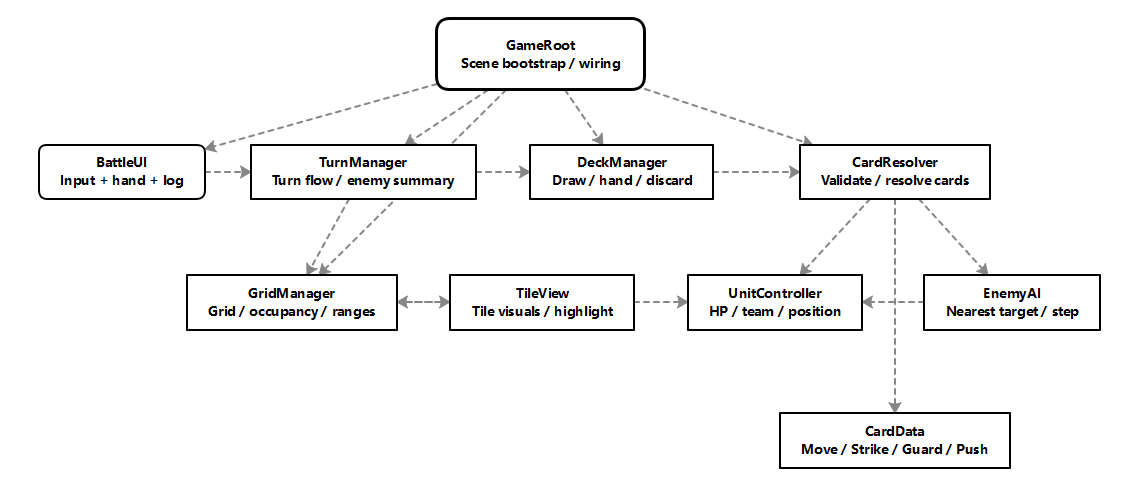
\includegraphics[width=0.93\textwidth]{media/architecture-diagram-wr1-style.png}
\caption{Current WR2 runtime architecture for the \projectname{} prototype}
\label{fig:architecture}
\end{figure}

At runtime, \texttt{GameRoot} wires the battle scene, \texttt{TurnManager} owns phase changes and card-play limits, and \texttt{BattleUI} collects player input. \texttt{DeckManager} controls draw, hand, and discard state, \texttt{CardResolver} resolves the four card types, \texttt{GridManager} owns tiles and reachability, and \texttt{UnitController} stores shared unit state. This is the full module set needed by the narrowed WR2 slice.

The WR1 to WR2 architecture carry-over can be summarised more explicitly as follows:

\begin{itemize}
\item \textbf{Inherited.} Separate responsibilities for turn flow, grid logic, cards, units, and UI still provide the clearest high-level structure for the demo.
\item \textbf{Modified for scope control.} The architecture now assumes one self-contained battle scene instead of a wider scene or campaign structure.
\item \textbf{Modified for traceability.} Player and enemy runtime state were collapsed into one shared \texttt{UnitController} with \texttt{TeamType}, which keeps health, guarding, and occupancy rules easier to explain.
\item \textbf{Modified for implementation speed.} Card behaviour is resolved in one explicit \texttt{CardResolver} rather than a generic effect hierarchy, matching the four-card WR2 scope.
\item \textbf{Modified for validation clarity.} \texttt{EnemyAI} stays deterministic and shallow so enemy turns are readable in demonstration and easier to verify against screenshots and logs.
\item \textbf{Modified for prototype practicality.} \texttt{BattleUI} uses a lightweight panel plus raycast input path, prioritising clarity and integration speed over a more polished UI stack.
\end{itemize}
